% !TEX TS-program = XeLaTeX
% use the following command:
% all document files must be coded in UTF-8
\documentclass[english]{textolivre}
% build HTML with: make4ht -e build.lua -c textolivre.cfg -x -u article "fn-in,svg,pic-align"

\journalname{Texto Livre}
\thevolume{15}
%\thenumber{1} % old template
\theyear{2022}
\receiveddate{\DTMdisplaydate{2022}{3}{11}{-1}} % YYYY MM DD
\accepteddate{\DTMdisplaydate{2022}{4}{19}{-1}}
\publisheddate{\today}
\corrauthor{Elias Said-Hung}
\articledoi{10.35699/1983-3652.2022.38733}
%\articleid{NNNN} % if the article ID is not the last 5 numbers of its DOI, provide it using \articleid{} commmand 
% list of available sesscions in the journal: articles, dossier, reports, essays, reviews, interviews, editorial
\articlesessionname{articles}
\runningauthor{Said-Hung et al.} 
%\editorname{Leonardo Araújo} % old template
\sectioneditorname{Daniervelin Pereira}
\layouteditorname{Carolina Garcia}

\title{Management and academic anxiety in Ibero-American higher institutions students during COVID-19}
\othertitle{Gestão e ansiedade acadêmica em estudantes de instituições superiores ibero-americanas durante a COVID-19}
% if there is a third language title, add here:
%\othertitle{Artikelvorlage zur Einreichung beim Texto Livre Journal}

\author[1]{Elias Said-Hung  \orcid{0000-0002-0594-5906} \thanks{Email: \url{elias.said@unir.net}}}
\author[2]{Eva Matarín Rodríguez-Peral \orcid{0000-0002-1701-3911} \thanks{Email: \url{eva.matarin@urjc.es}}}
\author[3]{Carolina Mejía Corredor\orcid{0000-0002-3560-5443}\thanks{Email: \url{cmejiaco@universidadean.edu.co}}}
\affil[1]{Universidad Internacional de La Rioja, Education Faculty, Logroño, Spain.}
\affil[2]{Rey Juan Carlos University, Faculty of Communication Sciences, Department of Communication Sciences and Sociology, Fuenlabrada, Madrid, Spain.}
\affil[3]{EAN University, Bogotá, Colombia.}

\addbibresource{article.bib}
% use biber instead of bibtex
% $ biber article

% used to create dummy text for the template file
\definecolor{dark-gray}{gray}{0.35} % color used to display dummy texts
\usepackage{lipsum}
\SetLipsumParListSurrounders{\colorlet{oldcolor}{.}\color{dark-gray}}{\color{oldcolor}}

% used here only to provide the XeLaTeX and BibTeX logos
\usepackage{hologo}

% if you use multirows in a table, include the multirow package
\usepackage{multirow}

% provides sidewaysfigure environment
\usepackage{rotating}

% CUSTOM EPIGRAPH - BEGIN 
%%% https://tex.stackexchange.com/questions/193178/specific-epigraph-style
\usepackage{epigraph}
\renewcommand\textflush{flushright}
\makeatletter
\newlength\epitextskip
\pretocmd{\@epitext}{\em}{}{}
\apptocmd{\@epitext}{\em}{}{}
\patchcmd{\epigraph}{\@epitext{#1}\\}{\@epitext{#1}\\[\epitextskip]}{}{}
\makeatother
\setlength\epigraphrule{0pt}
\setlength\epitextskip{0.5ex}
\setlength\epigraphwidth{.7\textwidth}
% CUSTOM EPIGRAPH - END

% LANGUAGE - BEGIN
% ARABIC
% for languages that use special fonts, you must provide the typeface that will be used
% \setotherlanguage{arabic}
% \newfontfamily\arabicfont[Script=Arabic]{Amiri}
% \newfontfamily\arabicfontsf[Script=Arabic]{Amiri}
% \newfontfamily\arabicfonttt[Script=Arabic]{Amiri}
%
% in the article, to add arabic text use: \textlang{arabic}{ ... }
%
% RUSSIAN
% for russian text we also need to define fonts with support for Cyrillic script
% \usepackage{fontspec}
% \setotherlanguage{russian}
% \newfontfamily\cyrillicfont{Times New Roman}
% \newfontfamily\cyrillicfontsf{Times New Roman}[Script=Cyrillic]
% \newfontfamily\cyrillicfonttt{Times New Roman}[Script=Cyrillic]
%
% in the text use \begin{russian} ... \end{russian}
% LANGUAGE - END

% EMOJIS - BEGIN
% to use emoticons in your manuscript
% https://stackoverflow.com/questions/190145/how-to-insert-emoticons-in-latex/57076064
% using font Symbola, which has full support
% the font may be downloaded at:
% https://dn-works.com/ufas/
% add to preamble:
% \newfontfamily\Symbola{Symbola}
% in the text use:
% {\Symbola }
% EMOJIS - END

% LABEL REFERENCE TO DESCRIPTIVE LIST - BEGIN
% reference itens in a descriptive list using their labels instead of numbers
% insert the code below in the preambule:
%\makeatletter
%\let\orgdescriptionlabel\descriptionlabel
%\renewcommand*{\descriptionlabel}[1]{%
%  \let\orglabel\label
%  \let\label\@gobble
%  \phantomsection
%  \edef\@currentlabel{#1\unskip}%
%  \let\label\orglabel
%  \orgdescriptionlabel{#1}%
%}
%\makeatother
%
% in your document, use as illustraded here:
%\begin{description}
%  \item[first\label{itm1}] this is only an example;
%  % ...  add more items
%\end{description}
% LABEL REFERENCE TO DESCRIPTIVE LIST - END


% add line numbers for submission
%\usepackage{lineno}
%\linenumbers

\begin{document}
\maketitle

\begin{polyabstract}
\begin{abstract}
The COVID-19 pandemic has caused uncertainty and instability in the population regarding the capacity of institutions to manage and mitigate its impact. In such an emergency, it is possible to ask how higher education institutions have dealt with this situation and what elements of institutional management have had the most significant influence in controlling stress and academic anxiety. The study aims to measure the level of academic anxiety among university students in Ibero-America since March 2020 due to the COVID-19 pandemic. It also seeks to identify the associated variables; some linked to the digital sphere, which affect the perception of the evaluation made by these students of the institutional management carried out by higher education institutions in Ibero-America. This article provides the quantitative research results that collected data using an anonymous online survey conducted from April 6 to April 24, 2020, in some higher education universities in Ibero-America, including 523 students surveyed. The data analysis is based only on the survey respondents' answers registered in institutions in six Ibero-American countries. The results identify psycho-social variables associated with the level of academic anxiety students perceive. They also point to the need for higher education institutions in Ibero-America to review their management models to guarantee their educational communities (e.g., students). This support consists of reinforcing soft skills that increase the capacity to transform the educational model.

\keywords{Higher education \sep Management \sep Students \sep Anxiety \sep COVID-19}
\end{abstract}

\begin{portuguese}
\begin{abstract}
A pandemia de COVID-19 causou incerteza e instabilidade na população em relação à capacidade das instituições de administrar e mitigar seu impacto. Em tal emergência, é possível perguntar como as instituições de ensino superior lidaram com essa situação e que elementos da administração institucional tiveram maior influência no controle do estresse e da ansiedade acadêmica. O objetivo deste estudo é medir o nível de ansiedade acadêmica entre os estudantes universitários na Ibero-América desde março de 2020, como resultado da pandemia de COVID-19. O estudo também procura identificar as variáveis associadas, algumas ligadas à esfera digital, que afetam a percepção da avaliação feita por esses estudantes da gestão institucional realizada pelas instituições de ensino superior na Ibero-América. Este artigo fornece os resultados quantitativos da pesquisa que coletou dados utilizando uma pesquisa \textit{on-line} realizada de 6 a 24 de abril de 2020 em algumas universidades de ensino superior da Ibero-América, incluindo um total de 523 estudantes pesquisados. A análise dos dados se baseia apenas nas respostas dos entrevistados da pesquisa registrados em instituições de seis países ibero-americanos. Os resultados identificam variáveis psicossociais associadas com o nível de ansiedade acadêmica percebido pelos estudantes. Eles também apontam para a necessidade de as instituições de ensino superior na Ibero-América reverem seus modelos de gestão a fim de garantir suas comunidades educacionais (por exemplo, estudantes). Esse apoio consiste em reforçar as competências transversais que aumentam a capacidade de transformar o modelo educacional.

\keywords{Educação superior \sep Administração \sep Estudantes \sep Ansiedade \sep COVID-19}
\end{abstract}
\end{portuguese}
% if there is another abstract, insert it here using the same scheme
\end{polyabstract}

\section{Introduction}

During the first semester of 2020, coronavirus SARS-CoV-2 produced a pandemic derived from COVID-19, hitting all social spheres, affecting the daily life routine of every single person, and profoundly affecting the hitherto existing use of technology. It has become an essential tool for maintaining educational and work activities and combating social isolation. At the time of this writing, this disease had already caused 449,750,235 cases of infection and 6,014,881 deaths by March 2022 \cite{johns_hopkins_university_covid-19_nodate}. Since March 2020, the world has seen how daily life activities have become dangerous because of the ease of contamination by the virus. The speed of transmission and spread of the virus and the severe consequences have led governments to implement COVID-19 prevention measures such as confinement and social isolation. These measures implemented by different governments have sometimes negatively affected families and even their mental health, which has not been included in decision-making models \cite[p.~801]{sonugabarke_editorial:_2021}. The consequences include psychological reactions of anxiety, depression, and even social panic due to the uncertainty of the situation \cite{rajkumar_covid-19_2020,yang_mental_2020}.

The confinement caused by Covid-19 generated an institutional context throughout the educational system of emergency. A reality that brought the challenge to adapt the educational models and institutional resources to guarantee the maintenance of the teaching-learning activities by teachers and students \cite{pardo_expandir_2021}. There was hardly any time to assume the particularities of the population related to the learning and teaching process, the digital culture in them, or the socio-sanitary and psychological context that each of them presented or which has affected the development of their work \cite{unesco_covid-19_2020,espino-diaz_analyzing_2020,kosir_predictors_2020}. They remarked on the increase of stress assumed by teachers and students to consider the reality experienced due to the pandemic and an increase in stress associated with their self-efficacy and attitudes towards virtual education and technology. It all happened within an institutional context with a marked difference in the level of support provided to these teachers, guaranteeing an essential protective factor that would help reduce stress \cite{brackett_emotion-regulation_2010}.

Stress is considered a disorder that emanates from the failure to adapt to an en-vironment where threats may be found \cite{selye_stress_1950}. The surroundings, the uncertain-ty, and the demands of societies that want to continue moving forward to return to the previous state of normalcy as soon as possible have become stressing issues for peo-ple. Stress and anxiety are very close, and sometimes it is challenging to separate con-cepts, as both are very complex. There is unanimous support when studying stress at an operative level that shows physiological aspects of stressful situations. In contrast, research projects about anxiety focus on subjective elements regarding reactions to stress \cite{sierra_ansiedad_2003}.

The uncertainty caused by COVID-19 affects all population sectors and is not in-different to the academic community. In this specific case, the students had to face the challenge of continuing their studies. The academic staff was challenged to ensure a minimum academic quality while adapting to the confinement because of COVID-19 \cite{garcia_aretio_saberes_2020}.

The uncertainty and instability context generated by COVID-19 has brought institutions to implement actions focused on strengthening their capacity to handle and diminish its impact. The higher institution's administration must cope with the decision-making and management of the available resources to reach an objective or solve a specific problem, improving their social capital or community resilience \cite{aparicio_capital_2017}.  The COVID-19’s pandemic has caused different levels of negative social impacts according to \textcite{turcaz_romero_intervencion_2016}, and \textcite{valdez_zepeda_public_2018}. In this context, higher education institutions had to assume their forma-tive mission and responsibility to social welfare, addressing the prevention of conse-quences caused by disasters such as the one experienced \cite{astudillo_pizarro_spatial_2019,perez_perez_service-learning_2019}. In such an emergency, it is possible to ask how higher education institutions have dealt with this situation and what elements of institutional management have had the most significant influence in controlling stress and academic anxiety.

\section{The impact of COVID-19 on education}

This sanitary problem has also affected the educational landscape. In this way, the educational administration deals with a set of actions and strategic decisions that include, on the one hand, administrative management and, on the other, institutional leadership, pedagogical management, and community management \cite{meza_revatta_gestion_2020}. Management offers the possibility of extending an organization's options to reach a goal. As \textcite[p.~57]{torres_pacheco_gestion_2015} said, "the actions that are integrated to achieve an objective at a certain time; it is the main action of the administration and the intermediate link between the concrete planning and objectives that need to be reached".% (p.57).

The effects caused by the COVID-19 pandemic on learning have been severe \cite{unicef_state_2021}. The number of students affected by school closures worldwide has exceeded 1.6 billion learners \cite{unicef_state_2021}. Some schools are still entirely closed, and others are only partially open. Thus, there are currently 117 million students affect-ed by the total closure of schools in 18 countries \cite{unesco_unesco_2021}. "Millions of children and youth are at risk of never returning to education" \cite[p.~5]{unicef_state_2021}. The isolation measures that have resulted in school closures have affected more than 616 million students \cite{unicef_covid:19_2022}. Continuous levels of stress and anxiety can affect students' academic performance \cite{fernandez_cruz_evaluation_2020,sanchez-gomez_inteligencia_2020,morales_rodriguez_diferencias_2021} by interfering with their attention span and their levels of concentration and retention of information \cite{jadue_algunos_2001}. Before COVID-19, studies on academic anxiety focused on students' difficulty adapting to their environment (social and family contexts). Other factors such as commuting and extracurricular activities were also considered \cite{balanza_galindo_prevalencia_2009}. Some significant differences have been identified in universities such as Universidad Católica San Antonio de Murcia, where different anxiety levels have been observed in their students \cite{balanza_galindo_prevalencia_2009}, the field of knowledge taught (Health Sciences and Business Legal Sciences).

Reactions to unexpected situations are adaptive strategies to deal with them. However, when these emotions are of great intensity, they are not beneficial to the individual, and instead of helping students adapt, they increase their perception of insecurity \cite{valero_cedeno_afrontamiento_2020}. Therefore, it is necessary to know the psychological impact that the pandemic is causing to promote strategies to diminish its effect within the educational sector. Research that has delved into the emotional and psychological impacts of COVID-19 and the coping measures shows that stress levels in the general population have increased \cite{barraza_macias_estres_2020,valiente_vida-covid-19_2020}.

Studies show that anxiety, stress, and depression have been overwhelmingly prevalent during COVID 19 \cite{shah_prevalence_2021,kar_stress_2021}. However, also al-low us to understand how social isolation affects the population's mental health around the world - e.g., China, Ecuador, Mexico, Saudi Arabia, Canada, and the United States, among others \cite{barraza_macias_estres_2020,wang_immediate_2020,joseph_immediate_2021,mautong_assessment_2021,turna_anxiety_2021}. The investigations conducted in China on the psychological impact produced by COVID-19 showed that "women and students experienced a psychological impact because of the infection and higher levels of stress, anxiety, and depression" \cite[p.~23]{wang_immediate_2020}. Furthermore, an analysis regarding its effect on Chinese college students revealed that 24.9\% of the survey respondents had experienced anxiety due to COVID-19 \cite{cao_psychological_2020}. The data collected by \textcite[p.~17]{barraza_macias_estres_2020} on what he called "Pandemic Stress" %(p.17) 
in the Mexican population show that the risk of being infected and the lack of trust in the healthcare system are factors that have increased the levels of stress during confinement. Some of the symptoms are high levels of anxiety and lack of sleep.

COVID-19's situation required urgent action and different activities in education. \textcite{unesco_covid-19_2020} promoted the Global Education Coalition for COVID-19, which aimed to improve learning processes (mediated by technology) in this health context. Several studies have focused on social-emotional skills as promoters of students' well-being, indicating that reducing stress requires helping students about the pandemic and equipping them with resources to manage their emotions \cite{salmelaaro_adolescents_2021}.

Some analyses of the strategies to face the situations of stress experienced by the educational community show that the measures to be implemented should be aimed at the internal strengthening of everyone \cite{valero_cedeno_afrontamiento_2020}. Teachers and students faced the challenge of promoting support measures, training, and learning soft skills. The \textcite{european_commission_recomendacion_2018} stated that social and emotional skills help individuals learn to react to uncertainty. "A higher degree of emotional regulation is related to a lower experience of stress factors" \cite[p.~12]{cuevas_lopez_emotional_2021}. These skills can also help cope with stressful situations; they need to be reinforced \cite{marrero_sanchez_habilidades_2018}.

Recent research indicates that adaptation to synchronous learning was perceived as more positive as self-perceived competence increased because the teacher then understood change as opportunity and success. Conversely, negative emotions surfaced when the teacher's self-perceived competence decreased \cite[p.~7156]{meishar-tal_times_2021}. The approaches of authors such as \textcite{villafuerte_rol_2020} aim to provide teachers with the appropriate tools to quickly adapt to the challenge of dealing with education during the pandemic and the role they must play during this time of supporting students learning. \Cref{Table01} shows the main characteristics that a teacher should develop.

\begin{table}[h!]
\centering
\caption{The Role of the Teacher in the COVID-19 Era for supporting student's learning.}
\label{Table01}
\begin{tabular}{p{0.3\textwidth}p{0.65\textwidth}}
\toprule
Role & Objective \\
\midrule
Support for Containment & Exceptional situations should not affect students emotionally. This role aims to protect students' mental health. \\
Promotion of Resilience & Making students capable of recovering from adverse situations provides them with training and the necessary tools. \\
Academic Guidance & Providing students with tools for their personal growth can develop guided skills that motivate them to resolve conflicts.\\
Opposition to Procrastination & Providing students with self-confidence, affection, and self-esteem so that they do not postpone their activities. \\
Active and empathetic listening & Trying to understand others. \\
Emotional Advisory & Ability to identify needs, work in teams, and keep an open mind to learning processes and fostering skills.\\
Institutional Advisory & Analysis and evaluation of the educational methodologies used to promote educational development. \\
Promotion & Achieving the intended educational objectives, taking into account the students' potential, context, and interests.\\
\bottomrule
\end{tabular}
\source{Prepared by the authors based on \textcite{villafuerte_rol_2020}.}
\end{table}

\textcite{villafuerte_rol_2020} show the relevance of those soft skills, in which empathy and the transmission of fairness play a fundamental role in overcoming unexpected situations that affect the educational system. Studying the psychological well-being of social confinement may have beneficial consequences for the general population \cite{florencia_vela_relajacion_2020}. It is necessary to learn the level of academic anxiety that the university community is experiencing and the associated variables during the pandemic. In this respect, some aspects related to the perception of relaxation could have an element of protection against the anxiety produced by the pandemic \cite{florencia_vela_relajacion_2020}.

The educational area does not yet know the real impact of COVID-19 on stu-dents' mental health. Still, researchers have noticed that this pandemic will affect, in general, long after the virus is finally controlled \cite{de_oliveira_araujo_impact_2020}. That is why it is necessary to continue promoting knowledge by adapting and innovating in the educational processes of learning and teaching. Studies developed by \textcite{odriozola-gonzalez_psychological_2020} in the Spanish university context show that anxiety, depression, and stress within the university community are higher among students than among staff. Some strategies for facing situations of stress and anxiety, such as those experienced in the pandemic, point to the necessity of promoting activities that favor a positive attitude. These actions are related to sharing activities with other people through digital tools that enable social contact despite social distancing, collaborating on social causes, or promoting collective leisure \cite{valero_cedeno_afrontamiento_2020}, i.e., activities that increase support and belonging a group.

Likewise, studies such as the one conducted by \textcite{iqbal_effect_2021} on the impact of emotional intelligence on academic performance during the COVID-19 pandemic indicate that fostering competencies linked to emotional intelligence improves academic performance. Specifically, it is advisable to train the dimensions of self-regulation and self-awareness since working on these aspects has significantly affected academic performance \cite{iqbal_effect_2021}. On the other hand, some of the management proposals that have been put forward in the educational context \cite{montes-rodriguez_ruta_2020} aim to promote more human organizational cultures, with communication channels that facilitate a greater closeness between the administrative area, teachers and students. Besides, active listening between students and teachers is also expected to consider emotional management and solutions to uncertainty. The pandemic context forced the educational sector to adapt its face-to-face learning processes to online processes, besides the challenge of including soft skills and support measures in the institutional management of public institutions to diminish the effects of COVID-19 on the educational sector.

As time progresses, there is a need to measure and minimize the impacts of the pandemic on students, including those related to disruptions in education \cite[p.~1]{almeida_editorial_2021}. Studies focused on the transition from face-to-face to virtual mode car-ried out in centers whose teaching process was not planned to face this period of uncertainty and emphasized how to execute the learning strategy while guaranteeing a similar level of quality. Online modality means not focusing on content but implementing active methodologies that use teamwork, such as the flipped classroom, a student-centered strategy, and synchronic sessions that facilitate social contact despite confinement \cite{de_vincenzi_aula_2020}. That is, actions aimed at designing learning experiences from institutional cooperative systems \cite{connor_chick_using_2020}, considering what has been stated in studies that highlight that enhancing digital competence and the skills to interact virtually with students is a fundamental aspect of avoiding social isolation \cite{fernandez_cruz_evaluation_2020}. This element would favor a training scenario more likely to reduce the stress levels associated with the socio-sanitary situation and state of confinement experienced with the Covid-19 Pandemic.

\section{Method}

The study's objective was to measure the level of academic anxiety in students and identify the variables associated with it that affect the perception of the Institutional management assessment led by higher education institutions in Ibero-America, since March 2020, because of the pandemic of COVID-19. The correlational study was de-signed under a non-experimental quantitative methodology, following different studies launched during the pandemic, like those carried out by \textcite{perez_escoda_digital_2021}, and \textcite{coronado_environmental_2021}, for example. The objective is also related to the hypothesis mentioned in this study: H1= The anxiety levels observed in the students were due to external and internal variables associated with the academic management faced by higher education institutions because of the pandemic scenario experienced in March 2020; H2= Higher institutions require an organizational culture based on the provision of soft skills and support measures that have allowed students to confront the pandemic scenario since March 2020.

This research was in line with the interest of other studies by authors such as \textcite{newbutt_possibility_2020}, \textcite{saez-delgado_caracterizacion_2020} or \textcite{luo_association_2022}, from different research approaches (e.g., psycho-social characterization of families during confine-ment, the importance of immersive technologies in vulnerable populations and the as-sociation between sociability and Covid-19 Pandemic stress), the socio-sanitary phe-nomenon, in general, and the educational system, from exploratory research such as the one shown in this article.

The results shown in this work are based on an online survey sent to professors and department managers of universities located in the countries studied, who were asked to participate in this study and invite their students to have an exploratory ap-proach to the topic addressed in the terms already exposed. The final random probabil-istic sample consisted of 523 sample units ($1-\alpha=95\%$ and $e=\pm 4.3$) between April 6 and 24, 2020. That is, data was collected during the first weeks of confinement in the coun-tries in Ibero-America analyzed because most of the higher education institutions in this study belong to these countries (Spain – 14th, 2020; Chile and Puerto Rico – March 19, 2020; and Argentina, Colombia, and Mexico – March 24, 2020).

The demographic and academic profile of the surveyed students (\Cref{Table02}) shows us a series of initial traits represented in the study sample, made up of: students (primarily undergraduate), women (66\% of students surveyed) aged between 20 and 41 years (mainly 28 years old), with an average of 3 household members who live with them, residents of urban areas, belonging to large urban centers, in which they went through the confinement that motivated this study (March and April 2020). The surveyed students are enrolled at the academic level, mainly in higher education institutions, based on a primarily face-to-face educational model. They spend an average of 5 hours a day developing their academic work.

\begin{table}[h!]
\begin{threeparttable}
\centering
\caption{Descriptive Aspects to Categorize Surveyed People.}
\label{Table02}
\begin{tabular}{p{0.22\textwidth} l *{5}{p{0.1\textwidth}}}
\toprule
Socio-Demographic Aspects & N & Minimum & Maximum & Mean & Median & Standard Deviation \\
\midrule
Age & 523 & 18 & 64 & 30.43 & 28 & 10.75 \\
Gender*	& 520 & 1 & 3 & 1.67 & 2 & 0.478 \\
Household Members & 523	& 1 & 7	& 3.35& 3 & 1.53 \\
Resident status in the city where the confinement is taking place\^{} & 523 & 1 & 2 & 1.09 & 1 & 0.289 \\
Size of the city of residence+ & 523 & 1 & 2 & 1.321 & 1 & 0.467 \\ 
Type of residence area++ & 523 & 1 & 2 & 1.82 & 2 & 0.386 \\
\midrule
Academic Aspects & N & Minimum & Maximum & Mean & Median & Standard Deviation \\
\midrule
Education model** & 522 & 1 & 2 & 1.40 & 1 & 0.490 \\
Average daily study time & 303 & 1 & 10 & 4.92 & 5 & 2.236 \\
Level of education currently training\^{}\^{}	& 523 & 1 & 3 & 1.52 & 1 & 0.544 \\
\bottomrule
\end{tabular}
\source{Prepared by the authors based on 523 samples analyzed.}
\begin{tablenotes}
\item [*] 1=Male / 2=Female / 3= Others 
\item [\^{}] 1=Yes / 2= No.
\item [+] 1=City of more than 100,000 inhabitants / 2= City of less than 100,000 inhabitants 
\item [++] 1=Rural / 2=Urban 
\item [**] 1=face-to-face educational model / blended or virtual educational model 
\item [\^{}\^{}] 1=Undergraduate / 2=Postgraduate / 3=Doctorate
\end{tablenotes}
\end{threeparttable}
\end{table}

Students surveyed were asked to rank from zero to ten on how they perceived the level of academic anxiety (dependent variable 1) and perception of the Institutional management assessment (dependent variable 2) carried out by higher education institutions at the time of this work. Both considered our dependent study variables. These variables were contrasted with independent variables obtained directly (using direct questions), related to aspects as shown in \Cref{Table03}.

\begin{table}[h!]
\centering
\begin{threeparttable}
\caption{Main independent variables considered to approach the proposed topic.}
\label{Table03}
\begin{tabular}{p{0.3\textwidth}p{0.6\textwidth}}
\toprule
Socio-health variables & Academic variables \\
\midrule
Level of social support perception and mood. & Educational modality in which he carried out his academic work before COVID-19. \\
Level of feeling at risk regarding COVID-19. & Level of assessment of the ICT resources made available by higher education entities during confinement.\\
Satisfaction level with social relationships. & Level of assessment on the academic barriers presented. \\
Level of exercise or development of healthy patterns or habits during confinement. & Level of assessment of the ICT equipment available in the home.\\
\bottomrule
\end{tabular}
\source{Prepared by the authors based on 523 samples analyzed.}
\end{threeparttable}
\end{table}

The applied survey (SPSS Statistics 20 was applied to data obtained in the online survey) was subject to the measurement of internal consistency to determine the variability of the information obtained in the independent variables through the questions asked to the respondents (\Cref{Table04}). The "$\alpha$" observed in most of these variables is acceptable (e.g., mood:  in this variable were considered: the feeling of nervousness, anxiety, anxiety's control, level of irritation, fear, or depression felt during the study period; academic area: questions such as study space (size), organization of working areas (including soundproofing, lighting, humidity, ventilation, and air quality, among others), and other living areas during confinement were considered; and educational barriers: in this variable questions related to problems during academic activity - e.g., constant interruptions by children, number of home tasks to be performed, and the lack of concentration, among other aspects - were considered \cite{loewenthal_introduction_1996,nunnally_psychometric_1978}. The "$\alpha$" observed in other variables (social support's perception: A 3-point Likert scale measured this variable (always, sometimes, never), as well as questions related to how many times students felt sad, lonely, happy, or beloved, among other aspects, during the study period; finally, healthy habits during the confinement, were also assessed: the healthy habits variable resulted from the answers given about routines done by students during the confinement (e.g., talking to friends or relatives, doing exercise, following a healthy and varied diet, and having hobbies, among others). A 5-point Likert scale measured this variable \cite{magnusson_teoritest_1978,nunnally_psychometric_1978}.

\begin{table}[h!]
\centering
\begin{threeparttable}
\caption{Study of Internal Consistency of Variables}
\label{Table04}
\begin{tabular}{lccccc}
\toprule
Variables & Indicator & N & Valid & Not valid & Cronbach's Alpha \\
\midrule
Healthy habits & 12 & 523 & 483 & 40 & 0.596 \\
Social support perception & 7 & 523 & 492 & 31 & 0.484 \\
Mood & 14 & 523 & 421 & 102 & 0.921 \\
Academic Area & 15 & 523 & 479 & 44 & 0.885 \\
Academic Barriers & 10 & 523 & 523& 0 & 0.638 \\
\bottomrule
\end{tabular}
\source{Prepared by the authors based on 523 samples analyzed.}
\end{threeparttable}
\end{table}

The asymmetric score given by respondents (\Cref{Figure01} and \Cref{Table05}) shows asymmetric values lower than 0. It is not usual in Social Science studies if we consider the number of sample units analyzed in this research \cite{rubio_hurtado_como_2012}, although this may not derive from the psycho-social context experienced by most of our respondents in the health crisis that caused the confinement. A context characterized by questions such as: how to proceed after COVID-19; what actions are effective for containing this illness; when the social distance measure applied by all the countries in the sample would end (e.g., some of them, such as Mexico, initially tried to avoid these measures). For this reason, we took the Kolmogorov-Smirnov (K-S) Test as a goodness-of-fit test at the level of the dependent variables taken for the study proposed in this work. The test shows us a significance of less than $.05$ ($p<.05$). Therefore, the distribution behaves against normality, and non-parametric statistics are more appropriate for approaching the subject studied (e.g., Kruskal-Wallis or Mann-Whitney U).

The use of non-parametric statistics was made to verify the difference in the scores of the means observed at the level of the categories of the study's variable. A variance between means may be due to own measurement errors of any social variable caused, for example, by circumstances associated with the respondent during his participation in the development of the applied survey \cite{urdanibia_error_2009}.

\begin{figure}[htbp]
\centering
\begin{minipage}{.8\textwidth}
\caption{Distribution graphs observed in study variables.}
\label{Figure01}
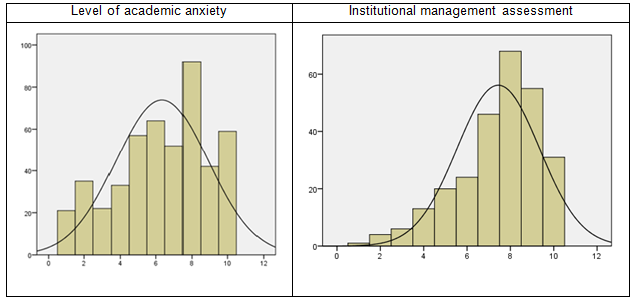
\includegraphics[width=\textwidth]{fig1.png}
\source{Prepared by the authors based on 523 surveys applied.}
\end{minipage}
\end{figure}

\begin{table}[h!]
\centering
\begin{threeparttable}
\caption{Descriptive and normality tests applied to the variable understudy.}
\label{Table05}
\begin{tabular}{p{0.2\textwidth}*{7}{c}}
\toprule
Variables & Valid & Nonvalid & Mean & Median & Asymmetry & Kurtosis & K-S Test \\
\midrule
Level of academic anxiety* & 477 & 46 & 6.34 & 7 & -0.415 & -0.754 & 3.156($p<.05$) \\
Institutional management assessment** & 268 & 255 & 7.44 & 8 & -0.870 & 0.420 & 3.114($p<.05$) \\
\bottomrule
\end{tabular}
\source{Prepared by the authors based on 523 samples analyzed.}
\end{threeparttable}
\end{table}
 
Given that the independent variables considered were measured in an ordinal way, Kendall's Tau-c Coefficient was used to measure their association with the dependent variables considered for the study of the proposed topic.

\section{Results}

From a psycho-social perspective, data collected showed an overall median val-uation of the respondents, mainly referring to the level of compliance with healthy hab-its ($3.34/5$ points and $\sigma=0.542$), the perception of risk of COVID-19 ($1.52/3$ points and $\sigma=0.542$), social support perception ($1.89/3$ points and $\sigma=0.318$) and mood ($2.99/5$ points and $\sigma=0.911$), and the level of satisfaction with relationships during the period analyzed ($3/5$ points and $\sigma=1.079$). The dispersion level observed in variables such as mood and satisfaction with relationships are also indicators of the high variation of op-tions given by the respondents. This fact helped us visualize in a better way the context they were facing when they answered the survey. It also helped us value the mood of the respondents and their satisfaction with relationships during the period of confinement, from the most extreme positions (good or bad) to those closer to the indicated median.

The socio-educational aspect also showed us a context of medium-high valuation at the level of spaces ($3.79/5$ points and $\sigma=0.853$). In addition, it allowed us to observe a favorable perception of the training barriers experienced at home (e.g., lack of concentration, demotivation, overwork, need to adapt to telework, care and interruptions of dependent children, and housework in charge). Moreover, data showed an upbeat assessment of the technological equipment (ICT) available for the exercise of the training work by the respondents ($3.84/5$ points and $\sigma=1.041$), despite the dispersion of the values reported by students, represented by the standard deviation registered in each of the variables above.

The data also showed us how 9 out of 10 students had laptops or desktops and smartphones. Still, only 4 out of 10 have helped fiber optics (more than 30 megabits). An aspect that would make it difficult to access content through digital resources that require much bandwidth, for example. Also, an aspect allows us to understand the level of valuation of digital resources (e.g., institutional mail, exam manager, virtual subject platforms, videoconference channels, and institutional digital repositories) made available to higher institutions to face the challenge of giving continuity to their training, in a confinement framework such as that experienced by students. It allowed us a context in which 7 out of 10 students considered the digital resources provided institutionally good or very good. However, institutional digital resources were not intensive (not considering the digital platform and email service) for the students surveyed because 5 out of 10 respondents said a context they sometimes use them.

Data collected, whereas the other five always do measure the perception of aca-demic anxiety (dependent variable 1) and the Institutional management assessment (dependent variable 2) during the period analyzed. The mean was $6.34/10$ and $7.44/10$ maximum points. Kendall's Tau-c coefficient (it is used to measure the association be-tween ordinal variables such as those analyzed here) allowed a low correlation ($p=0.025$) and inverse ($t=-0.164$) between the level of academic anxiety and the assess-ment of the higher institutions to which students enrolled at the time of carrying out this study. The level of academic anxiety was more elevated in students, and the perception of the institutional management assessment was lower.  

It can be possible to establish relationships by analyzing contingency tables dur-ing the statistical processing in this work between dependent and independent varia-bles. \Cref{Table06} shows a significant association ($p\leq 0.05$) of the academic anxiety observed in the students concerning the perception of healthy habits, social support, mood, and educational barriers, while the assessment that the students had about ICT resources and equipment available for the development of their training tasks. In the case of the perception of compliance with healthy habits during confinement, social support perception, the valuation of the digital resources available institutionally, and the technological resources available at a negative, weak but significant relationship. Meanwhile, training barriers at home would have a weak but positive association. At the same time, the state of mind perceived by the respondents would be the only variable with a moderate and positive association. There is an association where students' academic anxiety would be more significant in those cases with a lower capacity to recognize healthy habits than others who had a lower level of social support and valued less the digital resources provided by higher education institutions in the face of COVID-19.

\begin{table}[h!]
\centering
\begin{threeparttable}
\caption{Kendall's Tau-c coefficient for association studies in the variable anxiety.}
\label{Table06}
\begin{tabular}{lccc}
\toprule
Related variables & Valid & Tau-c & Sig \\
\midrule
Healthy habits & 473 & -0.122 & 0.000 \\
Social support’s perception & 473 & -0.112 & 0.001 \\
Mood & 466 & 0.392 & 0.000 \\
Academic Barriers & 432 & 0.164 & 0.000 \\
ICT resources & 427 & -0.121 & 0.001 \\
ICT equipment & 467 & -0.120 & 0.002 \\
\bottomrule
\end{tabular}
\source{Prepared by the authors based on 523 surveys applied.}
\end{threeparttable}
\end{table}

The results of the Kruskal-Wallis Test ($z(2)=8.859$, $p=0.012$) showed how the level of formative anxiety increased in students with a distribution of household chores that had risen during confinement compared with those who considered that such as-signments had not changed or had improved during the same period.

Regarding the assessment of institutional management (dependent variable 2), \Cref{Table07} showed a moderate association observed with mood and the perception of risk of contracting COVID-19. Therefore, the management's assessment faced by higher education institutions in Ibero-America would not be conditioned by variables directly related to the training tasks in charge but by external variables related to psycho-social aspects faced by students. Therefore, the assessment of institutional management will be higher when the students' mood is more favorable and a lower perception of con-tracting COVID-19.

\begin{table}[h!]
\centering
\begin{threeparttable}
\caption{Kendall's Tau-c coefficient for association studies in the variable Institutional management assessment.}
\label{Table07}
\begin{tabular}{lccc}
\toprule
Related variables & Valid & Tau-c & Sig \\
\midrule
Mood & 220 & -0.231 & 0.001 \\
Perception of risk to COVID-19 & 222 & 0.270 & 0.000 \\
\bottomrule
\end{tabular}
\source{Prepared by the authors based on 523 surveys applied.}
\end{threeparttable}
\end{table}

From the results of the Mann-Whitney Test ($z=8187$, $p=0.000$), the assessment of institutional management in the face of COVID-19 is lower among students whose educational model was eminently face-to-face compared to those whose training was blended or online. From the results of the Mann-Whitney Test ($z=8558.50$, $p=0.000$), the assessment of institutional management in the face of COVID-19 is lower among students whose educational model was eminently face-to-face compared to those whose training was blended or online.

Those mentioned above also happen when we analyze the perception of the risk of COVID-19 contagion. The results of the Kruskal-Wallis Test ($z(2)=8.613$, $p=0.003$ and $H(2)=9.111$, $p=0.011$, respectively) showed how students whose perception of risk is lower would have a more pessimistic assessment of the management faced by higher education institutions. At the same time, the review will be better among those who improved the perception of co-responsibility for household chores than others who feel it worst.

\section{Discussion and Conclusions}

Despite the limitations of the project, carried out at the beginning of the pandem-ic, like others already published \textcite{perez_escoda_digital_2021,coronado_environmental_2021}, this research has been able to meet the objec-tive of measuring the level of anxiety of university students. It has also identified the variables that affect the perception of the evaluation of the management carried out by Ibero-American higher education institutions during the COVID-19 pandemic.

The data showed that during the first weeks of lockdown caused by COVID-19, there were no high levels of academic anxiety. Emotional aspects and difficulties related to cohabitation at home have gained an incredibly relevant role in the educational context. For this reason, we should partially admit H1 of the study because, despite identified psycho-social and technological variables that have influenced the level of academic anxiety observed, students analyzed; did not identify variables associated with the educational management related to this issue.

On the other hand, H2 would be admitted in this work because higher institutions require an organizational culture based on the promotions of soft skills and support measures that allow students to confront the pandemic scenario lived since March 2020, above all, if we consider that the pandemic scenario will be present until all countries can apply vaccines to their populations. Only 14\% of the population had been vaccinated in Spain by May 2020 \cite{ministerio_de_sanidad_de_espana_vacuna_2021}. Ibero-America countries only have vaccines for less than 2\% of their population \cite{chevalier_cuantas_2021} and have not yet surpassed 25\% of the population inoculated with at least one dose \cite{pasquali_asi_2021}.

The situation lived since March 2020 makes Ibero-American countries analyzed to live with varying confinement levels (strict or more flexible) throughout the various waves of infection that have happened since then. It is a reality that requires reflecting on the educational models applied institutionally and how actions manage so that each academic community member can fully develop their functions. Variables identified in this study contributed to reality since March 2020 to the progressive increase of the deterioration of coexistence relationships during confinement. \textcite{florencia_vela_relajacion_2020} stated that the institutions' stakeholders should consider this.

The exposure must also be understood, considering the role that it would also be playing in favor of the levels of academic anxiety observed by the participants in this study and the different variables that affect it (academic barriers, digital resources, and ICT equipment). As we have seen in this study, variables helped to measure the emer-gency scenario experienced within the educational sector for higher education institu-tions and the students themselves. The perception of academy anxiety was related to training barriers and the availability of resources and technological equipment in their homes. This was something that conditioned the adequate performance of their aca-demic activities and responsibilities under a scenario that, as exponent authors such as \textcite{pardo_expandir_2021} points out, was characterized by: a high level of volunteerism; improvisation; and replication of technologically mediated educational experiences without having taken into account, at least during the period analyzed, neither the technological conditions, nor the socio-demographic and psycho-social profile, nor the perceptions that the students had about the pandemic scenario that motivated this work.

Beyond the improvement of the Covid-19 pandemic situation experienced since 2020 and the scenario provided by the data analyzed here at the beginning, we consider that the results shown will not lose validity in 2022. Above all, if we take into account the point of view of the accompaniment that higher education institutions must do with their students and when reflecting on the educational model, resources, and technological equipment applied to guarantee the training of their students.

The management of higher education institutions, especially those included in this project, has the challenge of supporting the most significant number of institutional members in their training activities' psycho-social and technological aspects. This sup-port process must begin with verifying the status of the conditions related to the varia-bles identified with the significant association in this work and culminate with the implementation of actions that benefit the academic practice of their students.

The management of educational institutions should focus on offering an institu-tional support framework more capable of dealing with new and potential challenges that must be faced from a social and educational point of view related to the approaches given by the \textcite{european_commission_recomendacion_2018} and by researchers such as \textcite{villafuerte_rol_2020}.

The Covid-19 Pandemic has been an event that has exposed the shortcomings that today exist in higher education institutions in terms of flexibility, agility, empathy, and implementation of actions aimed at strengthening their students' soft and digital skills. One of the lessons shown from the pandemic is that these institutions should improve their psycho-social support, adapt their educational models, and implement technological resources for the successful training of their students. The pandemic caused by the Covid-19, experienced since 2020, is still latent. That would improve the perception of higher education institutions by the population studied in future scenarios, such as those experienced in the period in which the data analyzed was collected.

Beyond the specific limitations of this exploratory research project and the ran-dom sample included for data collection, the findings emphasize the need to advance the lines of research on this topic. In addition, it highlights the need to promote research trends that analyze the subject in depth: considering the public or private nature of the institutions, their pedagogical approach (online, face-to-face, or mixed); and the degree of engagement of students and teachers, as well as for further research on the topic to be developed on the strategies that each institution can adapt to continue learning under these unknown and progressive scenarios, such as the current outbreak of COVID-19.  


\printbibliography\label{sec-bib}
% if the text is not in Portuguese, it might be necessary to use the code below instead to print the correct ABNT abbreviations [s.n.], [s.l.]
%\begin{portuguese}
%\printbibliography[title={Bibliography}]
%\end{portuguese}


%full list: conceptualization,datacuration,formalanalysis,funding,investigation,methodology,projadm,resources,software,supervision,validation,visualization,writing,review
\begin{contributors}[sec-contributors]
\authorcontribution{Elias Said-Hung}[conceptualization, datacuration, formalanalysis, investigation, methodology, projadm, supervision]
\authorcontribution{Eva Matarín Rodríguez-Peral}[conceptualization, formalanalysis]
\authorcontribution{Carolina Mejía Corredor}[conceptualization]
\end{contributors}


\end{document}

